\section{Experiments}
\label{sec:experiments}

% Budget: about 1.5 column-pages. This section carries required components 1 to 4.
% Rubric (4 pts): appropriate metrics, defended, comparison to the state of the art qualified.
% Source: distracted_driver.ipynb Section 6.1 (table_folds.csv) and Section 5.2 (driver probe).

We evaluate every model with 3-fold driver-grouped cross-validation and then score it once on the 4 frozen test drivers (Sec.~\ref{sec:data}). We report the cross-validation mean $\pm$ standard deviation alongside the test result. To measure how much driver identity survives in a network's visual features, we use a \emph{driver probe}, a separate classifier trained to guess which unseen driver appears in a frame from the model's frozen last-stage features. The probe is trained on classes \texttt{c0}--\texttt{c4} and tested on \texttt{c5}--\texttt{c9}, then the reverse. Frames from one video burst are nearly identical, so without this class split the probe could match a test frame to its near-duplicate in training instead of recognizing the driver. Lower probe accuracy means less driver identity remains.

%-------------------------------------------------------------------------
\subsection{Driver Leakage in Random Splits}
\label{sec:leakage}
% Source: Section 7, table_leakage_study.csv, table_leakage_group_split.csv, fig05.
A naive random frame split severely inflates performance on SFDDD (Table~\ref{tab:leakage_classical}). Because near-identical frames from the same video burst land in both training and validation, every model approaches ceiling accuracy under random splitting. Even the from-scratch CNN (\texttt{A-S}) and purely classical \texttt{HOG + RF} exceed 99\%. Under driver-disjoint folds, performance collapses sharply. \texttt{A-S} falls by 49.0 points ($0.997 \!\to\! 0.507$), \texttt{HOG + RF} drops by 40.4 points, and even ImageNet-pretrained \texttt{A-I} loses 14.3 points. Random-split scores therefore measure driver and cabin memorization rather than distraction recognition.

%-------------------------------------------------------------------------
\subsection{Classical Baselines versus CNNs}
\label{classical}
% Source: Section 12, Table/Figure 17.
% Where HOG + RF sits between A-S and A-I on unseen drivers. Whether body-centering helps
% the pose forest. What the deep network actually buys.
Comparing against non-neural classifiers shows what end-to-end convolutional learning actually adds (Table~\ref{tab:leakage_classical}). Hand-crafted HOG features generalize poorly to unseen drivers (0.590), yet they still beat the from-scratch CNN (0.507 for \texttt{A-S}), which overfits to cabin details when trained on only 14--15 drivers. Pose features do much better. A Random Forest on the 19 body-centered pose features reaches $0.795 \pm 0.011$, ahead of the same forest on raw image-centered keypoints (0.765) and of every from-scratch CNN, including \texttt{F-S} (0.693). Centering the keypoints on the shoulders removes seat position and body size before learning begins. ImageNet-pretrained CNNs are still the strongest overall, with 0.855 for \texttt{A-I} and 0.873 for \texttt{F-I} (0.927 on the test drivers). Where the pose forest sees only 9 upper-body joints, their visual features can tell apart the small objects that separate many classes, such as phones, cups, and cosmetics. 

% Placed where the text has reached page 4's right column, so it floats to the top of
% that column.
\begin{table}[t]
  \centering
  \small
  \caption{\textbf{Driver leakage and classical vs.\ CNN baselines.} Accuracy
  on a random frame split versus 3-fold driver-grouped cross-validation; the gap quantifies
  inflation from seeing the same drivers in training and validation.}
  \label{tab:leakage_classical}
  \setlength{\tabcolsep}{4pt}
  \begin{tabular}{@{}lccc@{}}
    \toprule
    Model & Random & Driver-grouped & Gap \\
    \midrule
    \texttt{A-S} (CNN, scratch) & 0.997 & $0.507 \pm 0.059$ & 0.490 \\
    \texttt{A-I} (CNN, ImageNet) & 0.997 & $0.855 \pm 0.051$ & 0.143 \\
    \texttt{HOG + RF} & 0.994 & $0.590 \pm 0.068$ & 0.404 \\
    \texttt{Pose (image) + RF} & 0.969 & $0.765 \pm 0.044$ & 0.205 \\
    \texttt{Pose (body) + RF} & 0.944 & $0.795 \pm 0.011$ & 0.149 \\
    \bottomrule
  \end{tabular}
\end{table}

% Full-width floats appear one page after their source, so this sits early to land on page 5.
\begin{table*}[t]
  \centering
  \small
  \caption{\textbf{Main ablation results.} Performance across 3-fold driver-grouped cross-validation (mean $\pm$ standard deviation over folds) and a single run on the four frozen test drivers. Models are initialized either from scratch (\texttt{-S}) or from ImageNet weights (\texttt{-I}). Probe is the driver probe defined in Sec.~\ref{sec:experiments}, where lower values indicate less driver identity (cross-validation chance is 0.137).}
  \label{tab:ablation_results}
  \setlength{\tabcolsep}{4pt}
  % Generated by figures/make_ablation_table.py from outputs/main/table_summary.csv and
% outputs/main/table_final_test.csv. Do not edit by hand, rerun the script instead.
\begin{tabular}{@{}llcccccccc@{}}
    \toprule
    & & \multicolumn{4}{c}{3-Fold Driver-Grouped Cross-Validation} & \multicolumn{4}{c}{Frozen Test (4 Drivers)} \\
    \cmidrule(lr){3-6} \cmidrule(l){7-10}
    ID & Configuration & Acc & Macro-F1 & Log-Loss & Probe & Acc & Macro-F1 & Log-Loss & Probe \\
    \midrule
    \texttt{A-S} & Baseline & $0.507 \pm 0.059$ & $0.505 \pm 0.054$ & $2.099 \pm 0.569$ & $0.796 \pm 0.054$ & $0.627$ & $0.609$ & $2.152$ & $0.715$ \\
    \texttt{B-S} & + GRL & $0.520 \pm 0.079$ & $0.522 \pm 0.082$ & $1.833 \pm 0.486$ & $0.823 \pm 0.040$ & $0.712$ & $0.696$ & $1.403$ & $0.789$ \\
    \texttt{C-S} & + Pose & $0.526 \pm 0.034$ & $0.527 \pm 0.028$ & $1.882 \pm 0.412$ & $0.827 \pm 0.028$ & $0.715$ & $0.694$ & $1.228$ & $0.677$ \\
    \texttt{D-S} & Full GRL & $0.544 \pm 0.097$ & $0.542 \pm 0.078$ & $1.770 \pm 0.633$ & $0.836 \pm 0.025$ & $\mathbf{0.734}$ & $\mathbf{0.709}$ & $1.255$ & $0.738$ \\
    \texttt{E-S} & + Confusion & $0.501 \pm 0.028$ & $0.503 \pm 0.042$ & $1.522 \pm 0.067$ & $\mathbf{0.668 \pm 0.041}$ & $0.675$ & $0.658$ & $1.125$ & $\mathbf{0.624}$ \\
    \texttt{F-S} & Full Conf.\ & $\mathbf{0.693 \pm 0.087}$ & $\mathbf{0.683 \pm 0.082}$ & $\mathbf{0.859 \pm 0.102}$ & $0.746 \pm 0.077$ & $0.713$ & $0.678$ & $\mathbf{0.844}$ & $0.723$ \\
    \midrule
    \texttt{A-I} & Baseline & $0.855 \pm 0.051$ & $0.853 \pm 0.051$ & $0.488 \pm 0.182$ & $0.713 \pm 0.073$ & $0.934$ & $0.923$ & $0.408$ & $0.558$ \\
    \texttt{B-I} & + GRL & $0.862 \pm 0.057$ & $0.859 \pm 0.057$ & $0.475 \pm 0.157$ & $0.589 \pm 0.100$ & $0.906$ & $0.883$ & $0.457$ & $0.551$ \\
    \texttt{C-I} & + Pose & $0.845 \pm 0.048$ & $0.842 \pm 0.048$ & $0.516 \pm 0.194$ & $0.585 \pm 0.069$ & $\mathbf{0.942}$ & $\mathbf{0.932}$ & $0.368$ & $0.561$ \\
    \texttt{D-I} & Full GRL & $\mathbf{0.874 \pm 0.038}$ & $0.870 \pm 0.038$ & $0.456 \pm 0.095$ & $0.550 \pm 0.071$ & $0.914$ & $0.899$ & $0.415$ & $0.636$ \\
    \texttt{E-I} & + Confusion & $0.856 \pm 0.057$ & $0.854 \pm 0.060$ & $0.502 \pm 0.159$ & $\mathbf{0.315 \pm 0.033}$ & $0.874$ & $0.870$ & $0.431$ & $\mathbf{0.379}$ \\
    \texttt{F-I} & Full Conf.\ & $0.873 \pm 0.021$ & $\mathbf{0.871 \pm 0.021}$ & $\mathbf{0.407 \pm 0.024}$ & $0.396 \pm 0.032$ & $0.927$ & $0.917$ & $\mathbf{0.286}$ & $0.389$ \\
    \bottomrule
\end{tabular}

\end{table*}

%-------------------------------------------------------------------------
\subsection{Ablation of the Adversary and Pose Fusion}
% Source: Sections 8.1 and 8.6, table_ablation_summary.csv, table_ablation_deltas.csv, fig16_ablation_summary.
% Main results table: CV accuracy, macro-F1, log-loss, probe (mean and std over folds) and
% test accuracy and macro-F1 for A to D, both initializations, plus the classical rows.
% Read every difference against the fold std and the "helped in k of 3 folds" count.
Three clear patterns emerge across the 12-model ablation ladder (Table~\ref{tab:ablation_results}). First, erasing driver identity \emph{alone} does not improve action recognition. Adding the confusion adversary leaves cross-validation macro-F1 essentially flat on both ImageNet and from-scratch runs, while ImageNet gradient reversal adds less than a point. Second, pairing the bounded confusion loss with body-centered pose fusion (\texttt{F-I}) outperforms either component alone. On ImageNet, \texttt{F-I} reaches the highest cross-validation macro-F1 at 0.871, gaining 1.8 points over the visual baseline and 2.9 points over pose alone, and the lowest log-loss at 0.407, while matching full GRL's accuracy with roughly half the fold-to-fold standard deviation ($\pm 0.021$ vs.\ $\pm 0.038$ for \texttt{D-I}, and under half that of all other ImageNet models). Finally, this balance holds on the four frozen test drivers, where \texttt{F-I} achieves 0.927 accuracy and 0.917 macro-F1 alongside the best probability calibration of any model (0.286 log-loss vs.\ 0.408 for the baseline), while cutting the driver probe to 0.389, well below both the baseline and full GRL.

\paragraph{ImageNet Pretraining versus From Scratch.}
% Source: distracted_driver.ipynb Section 10, table_init_comparison.csv,
% table_init_paired_delta.csv, table_results_per_fold.csv.
ImageNet initialization provides the single largest gain on unseen drivers. It raises cross-validation accuracy by 34.8 points over training from scratch (\texttt{A-I} vs.\ \texttt{A-S}) and shrinks the leakage drop from 49.0 to 14.3 points (Table~\ref{tab:leakage_classical}), since pretrained features keep a ResNet-18 from overfitting cabin textures on 14--15 drivers. Without pretraining, the confusion loss and pose fusion together close about half of that gap. The full from-scratch model (\texttt{F-S}) gains 18.6 points of accuracy over \texttt{A-S} ($0.507 \!\to\! 0.693$), cuts log-loss by more than half ($2.099 \!\to\! 0.859$), and beats every other from-scratch model in all 3 folds. It still trails ImageNet fine-tuning and the body-centered \texttt{Pose + RF}, however.

%-------------------------------------------------------------------------
\subsection{Scaling with the Number of Training Drivers}
\label{sec:scaling}
% Source: Section 11, scaling table, fig14_scaling.
% Answer both questions the instructions ask in one sentence each.
%   Where does it saturate? (or say it has not saturated at 22 drivers)
%   What would more data be worth? (the gain from the last step, with its spread)
% Whether D beats A when drivers are scarce.
\begin{figure*}[t]
  \centering
  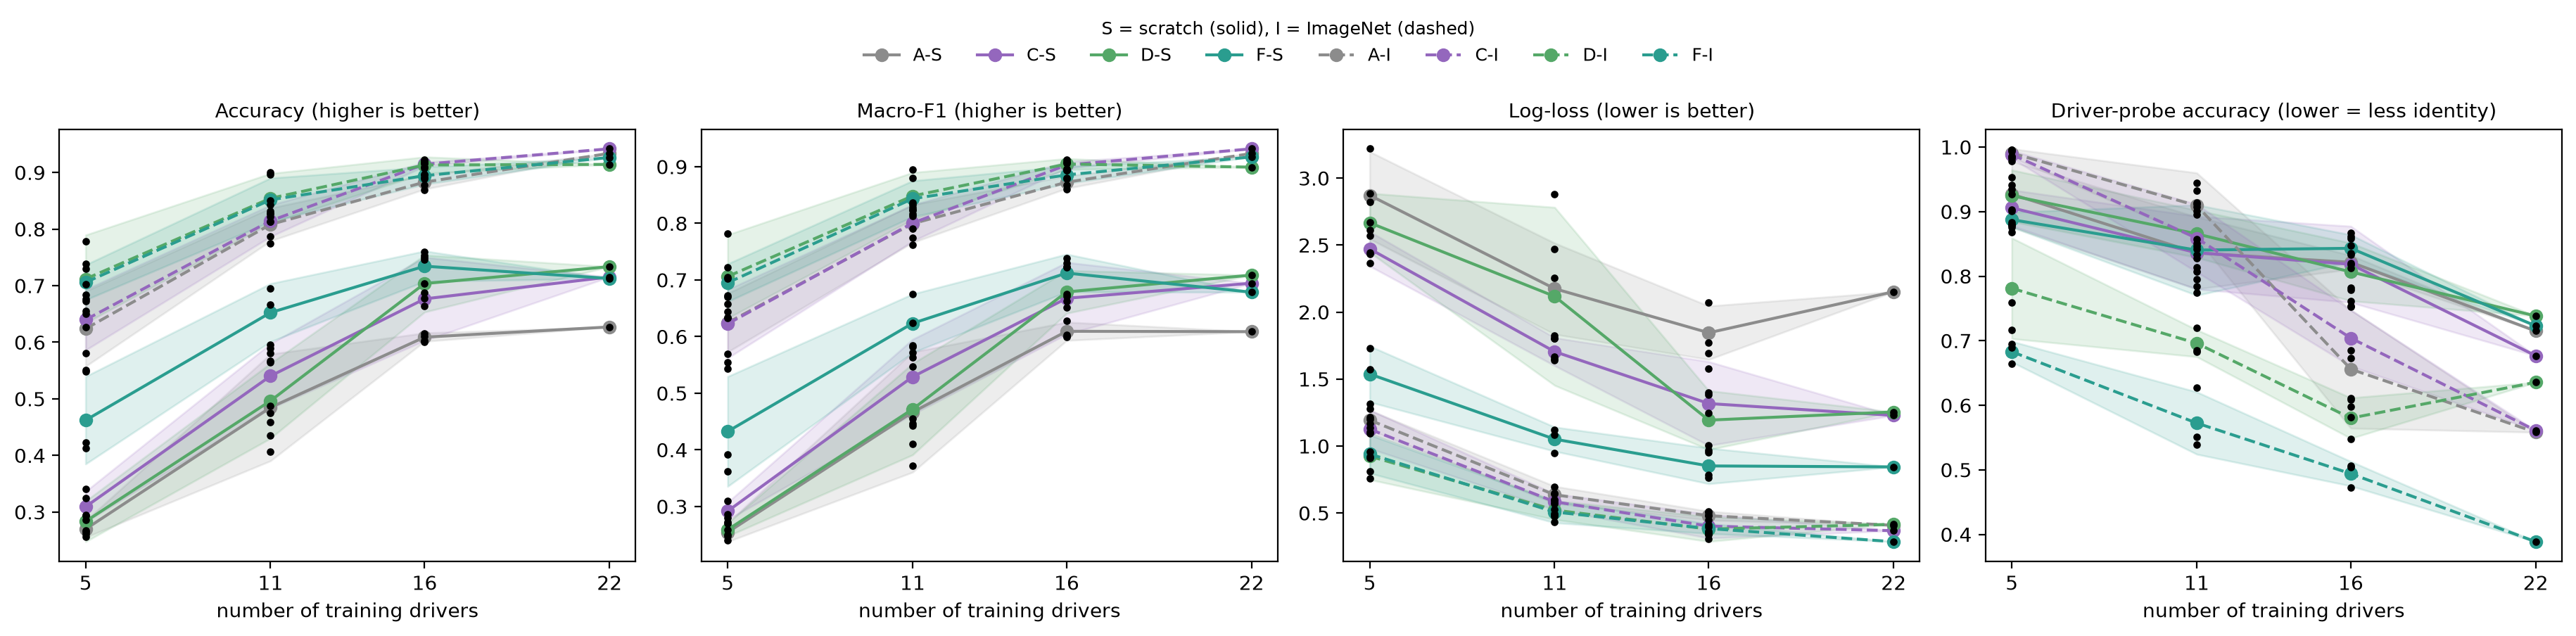
\includegraphics[width=\linewidth]{figures/fig14_scaling.png}
  \caption{\textbf{Scaling with the number of training drivers.} Test-driver accuracy, macro-F1, log-loss, and driver-probe accuracy for \texttt{A}, \texttt{C}, \texttt{D}, and \texttt{F}, from scratch (solid) and ImageNet (dashed). We omit \texttt{B} and \texttt{E} to limit compute, since Table~\ref{tab:ablation_results} shows that removing identity alone barely changes accuracy. Lines show means over random driver subsets, shaded bands one standard deviation, and dots individual runs (22 drivers is the single final model from Table~\ref{tab:ablation_results}).}
  \label{fig:scaling}
\end{figure*}

Figure~\ref{fig:scaling} tracks frozen-test performance as the training pool grows from 5 to 22 drivers (25\%--100\% of the development set). Pose fusion and adversarial regularization help most when driver diversity is scarce. With only 5 training drivers, the ImageNet baseline memorizes identity almost completely (0.991 probe) and falls to 0.624 test accuracy. Under the same 5-driver regime, combining pose fusion with an adversary lifts ImageNet accuracy by more than 8 points, reaching 0.712 with GRL and 0.706 with confusion loss (\texttt{F-I}), which also halves the run-to-run standard deviation and lowers the probe to 0.683. The gain is even starker from scratch, where \texttt{F-S} nearly doubles baseline accuracy (0.462 vs. 0.270). Although accuracy gaps narrow by 16 drivers, \texttt{F-I} retains a steady 0.16--0.34 probe advantage at every training size. Performance has not saturated at 22 drivers. Moving from 16 to 22 drivers still adds 5.1 points for the baseline and 3.3 points for \texttt{F-I}, so additional training drivers would likely improve accuracy further.

%-------------------------------------------------------------------------
\subsection{Adversary Design and Robustness}
\label{sec:robustness}
% Sources: Section 8.5 (table_final_test.csv, per-test-driver accuracy, fig15), Section 8.2 (fig10 driver probe), Section 9 (fig12).
% Spread of accuracy across the four test drivers. Whether the adversary lowers the probe.
% The adversarial study (adversarial_study.ipynb) goes here in one or two sentences, with
% details in the supplementary material.
To diagnose why standard gradient reversal (\texttt{B-I}) barely reduced driver identifiability in Table~\ref{tab:ablation_results}, and to choose our final adversary without touching the test set, we screened candidate designs on ImageNet ResNet-18 (Fold~0). Each candidate was scored with the worst case of class-split linear and MLP driver probes. Promising designs and mechanism checks were then confirmed with fresh multi-seed runs on 3 and 5-fold driver-grouped cross-validation
(Table~\ref{tab:adv_ablation}).

\begin{table}[t]
  \centering
  \small
  \caption{\textbf{Adversarial design ablation (ImageNet ResNet-18).} Screening rows report the Fold~0 worst-case linear/MLP driver probe, where lower is better, and macro-F1. On Fold~0, chance is 0.143 and always guessing the most common driver scores 0.195 (the majority floor). Untrained anchors use the hardened multi-split probe on 5 folds, and 5-fold confirmation rows average fresh seeds (chance 0.230).}
  \label{tab:adv_ablation}
  \setlength{\tabcolsep}{4pt}
  \begin{tabular}{@{}llcc@{}}
    \toprule
    Stage & Variant & Probe & Macro-F1 \\
    \midrule
    \multicolumn{4}{@{}l}{\textit{Untrained anchors (5-fold multi-split probe)}} \\
    Anchor & Random init & 0.999 & --- \\
    Anchor & Frozen ImageNet & 1.000 & --- \\
    \midrule
    \multicolumn{4}{@{}l}{\textit{Fold-0 screening (single-factor changes)}} \\
    Ref. & Baseline (no adversary) & 0.627 & 0.881 \\
    Ref. & GRL ($\lambda{=}1$, DANN ramp) & 0.607 & 0.884 \\
    Head & GRL, 2 head steps & 0.547 & 0.880 \\
    Strength & GRL, $\lambda{=}10$ & 0.577 & 0.876 \\
    Loss & Confusion, $\lambda{=}1$ (last stage) & \textbf{0.388} & 0.868 \\
    Loss & Confusion, $\lambda{=}3$ (last stage) & 0.333 & 0.841 \\
    Stages & Conf.\ $\lambda{=}3$, last 2 stages & 0.375 & 0.790 \\
    \midrule
    \multicolumn{4}{@{}l}{\textit{Mechanism, post-hoc, and 5-fold confirmation}} \\
    Mech. & GRL ensemble + head resets & 0.809 & --- \\
    Post-hoc & Baseline + forced INLP & 0.593 & --- \\
    \mbox{5-fold} & Baseline, no pose & 0.674 & 0.860 \\
    \mbox{5-fold} & Confusion $\lambda{=}1$, no pose & \textbf{0.446} & 0.857 \\
    \mbox{5-fold} & Confusion $\lambda{=}1$ + pose & 0.450 & \textbf{0.878} \\
    \bottomrule
  \end{tabular}
\end{table}

\paragraph{Baseline Identity Levels and Why GRL Fails.}
% Source: adversarial_study.ipynb Sections 3, 4, 5, 11 (outputs/adversarial/table_s3_anchors.csv,
% table_s3_reference.csv, table_s4_head.csv, table_s5_lambda.csv, table_s11_ensemble.csv).
Before fine-tuning, both frozen ImageNet and randomly initialized ResNet-18 features identify held-out drivers nearly 100\% of the time across disjoint action classes (Table~\ref{tab:adv_ablation}), showing that raw color and cabin textures uniquely fingerprint each subject. Standard fine-tuning lowers the driver probe to 0.627 on Fold~0 and 0.674 across 5 folds. Gradient reversal does only slightly better. Across deeper heads, $3\times$ head learning rates, extra head updates, penalty weights up to $\lambda{=}10$, constant ramps, multi-stage heads, and ensembles, the probe never drops below 0.547, and periodically resetting the head makes it worse (0.809). The cause is that gradient reversal rewards making the driver head wrong, not uncertain. The backbone learns to make the head confidently pick the wrong driver, so the head itself is right only 9.5\% of the time. The identity is still present, just relabeled, and a fresh linear probe trained on the same features still names the training drivers 67.7\% of the time.

\paragraph{Bounded Confusion Loss and Alternatives.}
% Source: adversarial_study.ipynb Sections 6, 7, 8, 12, 13, 14, 15 (table_s6_confusion.csv,
% table_s7_stages.csv, table_s8_augmentation.csv, table_s12_extended.csv, table_s13_inlp.csv,
% table_s14_probe_hardening.csv, table_s15_confirm5.csv, table_s15_hardened.csv).
Switching from GRL to the bounded uniform confusion loss ($\lambda{=}1$) on
the last stage resolves this failure mode. A uniform guess is the best the backbone
can reach, so it has no reason to make the head confidently wrong. On Fold~0, it cuts the driver probe to
0.388 while keeping macro-F1 within 0.02 of the baseline, whereas stronger penalties
($\lambda{=}3$) or earlier-stage heads degrade macro-F1
(Table~\ref{tab:adv_ablation}). Confirmed across 5 folds with fresh seeds,
last-stage confusion loss drives training-driver identity down to chance and cuts
the held-out probe by 22.8 points (0.446 vs.\ 0.674). That removes
over 60\% of the driver identity signal above the majority-class floor while
leaving macro-F1 virtually unchanged (0.857 vs.\ 0.860). Stricter checks using
multi-split, wide MLP, and $k$-NN probes show matching drops, confirming that
driver cues are genuinely erased rather than merely hidden from a linear
classifier. Finally, non-adversarial alternatives fall short. Neither heavy
appearance augmentation nor projecting out driver directions after training
via Iterative Nullspace Projection (INLP, 0.593) matches confusion
training.

% Placed where the text has reached page 6's right column, so it floats to the top of
% that column on the same page as the SOTA section.
\begin{table}[t]
  \centering
  \footnotesize
  \caption{\textbf{Comparison with published SFDDD methods by split protocol.} All rows evaluate on SFDDD; because held-out driver subsets vary across papers, scores are not directly comparable. NLL denotes multi-class log-loss where reported.}
  \label{tab:sota}
  \setlength{\tabcolsep}{3.5pt}
  \begin{tabular}{@{}llcc@{}}
    \toprule
    Method & Split Protocol & Acc & NLL $\downarrow$ \\
    \midrule
    \multicolumn{4}{@{}l}{\textit{Random frame splits (driver leakage)}} \\
    ViT-DD~\cite{ma2024vitdd} & Random (70/30) & 0.996 & 0.017 \\
    Ours (\texttt{A-I}, naive) & Random (67/33) & 0.997 & 0.013 \\
    \midrule
    \multicolumn{4}{@{}l}{\textit{Driver-disjoint splits (unseen drivers)}} \\
    Hssayeni \etal~\cite{hssayeni2017} (ResNet-152) & Driver-disj. & 0.850 & --- \\
    MobileNetV3-L~\cite{essahraui2026} & Driver-disj. & 0.889 & --- \\
    DEWS-EfficientNet~\cite{zhangCrossDriver} & Driver-disj. & 0.890 & --- \\
    Anchor-ViT~\cite{doshiAnchorVIT} & SFDDD val.$^\star$ & 0.923 & --- \\
    ViT-DD~\cite{ma2024vitdd} & Driver-disj.\ (18/6) & 0.925 & 0.397 \\
    Ours (\texttt{F-I}) & 3-fold driver-disj. & 0.873 & 0.407 \\
    Ours (\texttt{F-I}) & Driver-disj.\ (22/4) & 0.927 & 0.286 \\
    \bottomrule
    \multicolumn{4}{@{}l}{\scriptsize $^\star$Validation accuracy (92.4\% F1).}
  \end{tabular}
\end{table}

\paragraph{Effect on Unseen-Driver Robustness.}
% Source: adversarial_study.ipynb Sections 15, 16, 17 (table_s15_pose5.csv, table_s15_pose_fcls.csv,
% table_s16_test_delta.csv, table_s17_decoupling.csv), distracted_driver.ipynb Section 8.3b
% (table_error_by_driver.csv).
Across 105 visual-only 5-fold runs, lower driver identifiability alone does
not predict higher macro-F1 (slope $+0.036$, 95\% CI $[-0.016, +0.069]$). Its
practical payoff emerges when paired with pose fusion and on the hardest
unseen subjects. Across 5 folds, confusion loss plus pose cuts the visual
driver probe by 22.3 points to 0.450 while lifting macro-F1 by 1.8 points to
0.878 over the visual baseline (95\% CI $[+0.008, +0.027]$). On the four
frozen test drivers across three seeds, it lowers the driver probe by 13.1
points (0.420 vs.\ 0.551) and cuts log-loss by 0.115 (0.309 vs.\ 0.424) at
$0.917 \pm 0.002$ macro-F1. Most notably, in the main study \texttt{F-I} cuts
error rates on the two hardest development drivers (\texttt{p072} and
\texttt{p081}) by 27.2 and 25.6 points relative to the visual
baseline.

%-------------------------------------------------------------------------
\subsection{Comparison to the State of the Art}
\label{sec:sota}
% Source: published numbers from the cited papers (see Sec. 2). Our rows from
% table_leakage_study.csv, table_summary.csv, and table_final_test.csv.

Table~\ref{tab:sota} compares our final model against representative SFDDD
benchmarks grouped by split protocol. Because studies differ in held-out
drivers and fold schemes, absolute accuracies are \emph{not} directly
comparable across papers, and we do not claim to beat the state of the art.

Under random frame splits, published SFDDD models routinely exceed 99\%
accuracy (e.g., ViT-DD~\cite{ma2024vitdd} at 99.6\%, CAT-CapsNet~\cite{mittal2023catcaps}
at 99.9\%), matching our naive ImageNet baseline (\texttt{A-I}, 99.7\%) and
confirming that random splits primarily measure driver leakage
(Sec.~\ref{sec:leakage}). Under driver-disjoint splits, published accuracy
drops to 85--92.5\%. Transfer-learned ResNet-152~\cite{hssayeni2017} sits at
85.0\% (matching our \texttt{A-I} cross-validation baseline at 85.5\%), while recent
unseen-driver CNNs~\cite{zhangCrossDriver,essahraui2026} reach $\sim$89\%. The
highest scores come from heavier Vision Transformers that localize upper-body
or facial cues. Anchor-ViT~\cite{doshiAnchorVIT} reaches 92.3\% via learned
spatial anchors, and ViT-DD~\cite{ma2024vitdd} reaches 92.5\% (0.397 NLL) via
face crops and multi-task emotion labels. Our \texttt{F-I} model achieves
competitive accuracy and strong calibration (0.873 accuracy and 0.407 log-loss in cross-validation,
0.927 and 0.286 on test) on a single ResNet-18 backbone by pairing 19-d
body-centered pose fusion with a training-only uniform confusion loss,
complementing recent camera-view disentanglement work~\cite{celona2026dbmnet}
by directly erasing and verifying driver invariance.
